% !TeX program = pdflatex
\documentclass[12pt, a4paper]{article}

% ============================================================
% CẤU HÌNH TIẾNG VIỆT CHUẨN VÀ AN TOÀN CHO PDFLATEX
% ============================================================
\usepackage[utf8]{inputenc}
\usepackage[vietnam]{babel}
\usepackage[T5]{fontenc} 

% -- Toán học cơ bản & Nâng cao --
\usepackage{amsmath, amssymb, amsthm}
\usepackage{mathtools}

% -- Định dạng trang --
\usepackage[top=2.5cm, bottom=2.5cm, left=3cm, right=2.5cm]{geometry}
\usepackage{setspace}
\setstretch{1.3}
\usepackage{parskip}
\usepackage{enumitem}

% -- Đồ họa & Hình ảnh --
\usepackage{graphicx}
\usepackage{float}
\usepackage{caption}
\captionsetup{font=small, labelfont=bf}

% -- Bảng biểu dữ liệu --
\usepackage{booktabs}
\usepackage{array}
\usepackage{tabularx}
\usepackage{longtable}

% -- Tiêu đề trang & Định dạng Section --
\usepackage{fancyhdr}
\usepackage{titlesec}

\pagestyle{fancy}
\fancyhf{}
\rhead{\small Mô hình hóa thống kê}
\lhead{\small Các giả định quan trọng của mô hình hồi quy bội}
\cfoot{\thepage}
\renewcommand{\headrulewidth}{0.4pt}

\titleformat{\section}[block]
{\large\bfseries}
{\thesection.}{0.5em}{}[{\titlerule[0.4pt]}] 

\titleformat{\subsection}[block]
{\normalsize\bfseries}
{\thesubsection.}{0.5em}{}

% -- Cấu hình liên kết Hyperlinks --
\usepackage{hyperref}
\hypersetup{
	colorlinks=true,
	linkcolor=black,
	citecolor=black,
	urlcolor=black
}

% ============================================================
% BEGIN DOCUMENT
% ============================================================
\begin{document}
	
	% ============================================================
	% TITLE PAGE
	% ============================================================
	\begin{titlepage}
		\centering
		\vspace*{1.5cm}
		
		{\Large\bfseries Mô Hình Hóa Thống Kê}\\[0.5cm]
		{\rule{\linewidth}{1.5pt}}\\[0.3cm]
		
		{\Huge\bfseries
			Chủ đề 3: Các Giả Định Quan Trọng \\[0.3cm]
			Của Mô Hình Hồi Quy Bội}\\[0.3cm]
		{\rule{\linewidth}{1.5pt}}
		
		\vspace{2.5cm}
		
		\centering \large
		\renewcommand{\arraystretch}{1.5}
		\begin{tabular}{ll}
			\textbf{Môn học:} & Mô hình hóa thống kê \\
			\textbf{Giảng viên:} & TS. Nguyễn Thị Mộng Ngọc \\
			\textbf{Nhóm thực hiện:} & NHÓM 1
		\end{tabular}
		
		\vfill
		\textbf{Thành viên thực hiện:} \\[0.4cm]
		\renewcommand{\arraystretch}{1.3}
		\begin{tabular}{l c}
			\toprule
			\textbf{Họ và tên} & \textbf{Mã học viên} \\ 
			\midrule
			NGUYỄN NHẬT QUANG & 25C23002 \\
			PHẠM ĐOÀN VỊNH NGHI & 25C23012 \\
			LÊ HOÀNG NHƯ & 25C23014 \\
			\bottomrule
		\end{tabular}
		
		\vfill
		{\small Trường Đại học Khoa học Tự Nhiên - ĐHQGHCM}
	\end{titlepage}
	
	% ============================================================
	% PHÂN CÔNG CÔNG VIỆC
	% ============================================================
	\newpage
	\begin{center}
		{\Large\bfseries BẢNG PHÂN CÔNG NHIỆM VỤ VÀ ĐÁNH GIÁ}\\[0.3cm]
		{\rule{\linewidth}{1pt}}
	\end{center}
	
	\vspace{0.5cm}
	
	\begin{table}[h]
		\centering
		\small
		\renewcommand{\arraystretch}{1.4}
		\begin{tabularx}{\textwidth}{|l|c|X|c|}
			\hline
			\textbf{Họ và tên} & \textbf{Mã học viên} & \multicolumn{1}{c|}{\textbf{Nhiệm vụ thực hiện}} & \textbf{Đánh giá} \\
			\hline
			NGUYỄN NHẬT QUANG & 25C23002 & Tính tuyến tính; Tính chuẩn \& Tổng hợp file báo cáo; Thuyết trình & 100\% \\ \hline
			PHẠM ĐOÀN VỊNH NGHI & 25C23012 & Tính độc lập \& Phân công nhiệm vụ; Soạn câu hỏi thảo luận; Thuyết trình & 100\% \\ \hline
			LÊ HOÀNG NHƯ & 25C23014 & Tính đồng nhất phương sai \& Lập dàn ý công việc; Tổng hợp, kết luận; Thuyết trình & 100\% \\
			\hline
		\end{tabularx}
	\end{table}
	
	% ============================================================
	% TABLE OF CONTENTS
	% ============================================================
	\newpage
	\tableofcontents
	\newpage
	
	% ============================================================
	% SECTION 1: TỔNG QUAN
	% ============================================================
	\section{Tổng quan}
	
	\subsection{Hồi quy}
	Dựa vào nghiên cứu của Weisberg trong tài liệu \textit{Applied Linear Regression} \cite{weisberg2014}, hồi quy là một phương pháp thống kê nền tảng được dùng để mô hình hóa và định lượng mối quan hệ giữa biến phản ứng ($Y$) và một hoặc nhiều biến tiên đoán ($\mathbf{X}$). Nền tảng toán học của hồi quy dựa trên Hàm kỳ vọng có điều kiện (Conditional Expectation Function - CEF), ký hiệu là $E(Y|\mathbf{X})$, biểu thị giá trị trung bình của $Y$ tại các mức giá trị cố định của $\mathbf{X}$. Khái niệm hồi quy bắt nguồn từ công trình của Sir Francis Galton vào cuối thế kỷ 19, khi ông quan sát hiện tượng chiều cao của các thế hệ "hồi quy về mức trung bình" \cite{galton1886}. Ngày nay, mục đích chính của hồi quy bao gồm:
	\begin{itemize}
		\item Mô tả và định lượng mối quan hệ thống kê giữa các biến số.
		\item Dự báo giá trị của biến phản ứng dựa trên tập hợp biến giải thích.
		\item Kiểm soát các biến gây nhiễu theo nguyên lý \textit{ceteris paribus} (giữ các yếu tố khác không đổi).
	\end{itemize}
	
	\subsection{Mô hình hồi quy và Tính chất cốt lõi}
	Dựa vào nghiên cứu của James và cộng sự \cite{james2013}, mô hình hồi quy là biểu diễn toán học chính thức cho hàm $f(X)$. Dạng cơ bản nhất là Hồi quy tuyến tính đơn (SLR):
	\begin{equation}
		Y_i = \beta_0 + \beta_1 X_i + \varepsilon_i
	\end{equation}
	Trong đó: $\beta_0$ và $\beta_1$ là các tham số dân số cần ước lượng, và $\varepsilon_i$ là sai số ngẫu nhiên biểu diễn những biến thiên không giải thích được. Các tính chất cốt lõi bao gồm:
	\begin{itemize}
		\item \textbf{Phần dư ($\hat{e}_i$)}: Sự chênh lệch giữa giá trị quan sát thực tế và giá trị dự báo mẫu ($\hat{e}_i = y_i - \hat{y}_i$).
		\item \textbf{Hệ số xác định ($R^2$)}: Đo lường tỷ lệ phương sai của biến phản ứng $Y$ được giải thích bởi các biến độc lập trong mô hình.
	\end{itemize}
	
	\subsection{Hồi quy bội}
	Dựa vào tài liệu \textit{Linear Models with R} \cite{faraway2016}, hồi quy bội mở rộng cấu trúc tuyến tính đơn cho trường hợp có nhiều hơn hai biến tiên đoán ($p \geq 2$) nhằm kiểm soát tác động đồng thời của nhiều yếu tố và hạn chế thiên lệch do bỏ sót biến. Khi làm việc với mô hình hồi quy bội, cần đặc biệt lưu ý:
	\begin{itemize}
		\item \textbf{Kiểm định F toàn cục}: Dùng để đánh giá xem có ít nhất một biến giải thích tác động có ý nghĩa lên $Y$ hay không.
		\item \textbf{Kiểm định t từng phần}: Đánh giá đóng góp biên của từng hệ số.
		\item \textbf{Đa cộng tuyến (Multicollinearity)}: Hiện tượng các biến độc lập có tương quan mạnh với nhau, làm hệ số ước lượng kém ổn định.
	\end{itemize}
	
	\subsection{Mô hình hồi quy bội dạng ma trận}
	Dựa vào nghiên cứu của Rencher và Schaalje \cite{rencher2008}, mô hình hồi quy tuyến tính đa biến được biểu diễn thanh lịch dưới dạng đại số tuyến tính:
	\begin{equation}
		\mathbf{y} = \mathbf{X}\boldsymbol{\beta} + \mathbf{e}, \quad E(\mathbf{e}) = \mathbf{0}, \quad \text{Cov}(\mathbf{e}) = \sigma^2 \mathbf{I}_n
	\end{equation}
	Trong đó: $\mathbf{X}$ là ma trận thiết kế có kích thước $n \times (k+1)$ với cột đầu tiên là vectơ cột 1, $\mathbf{y}$ là vectơ cột của biến phản ứng, và $\boldsymbol{\beta}$ là vectơ các tham số hệ số. Để hệ phương trình chuẩn có nghiệm duy nhất, ma trận $\mathbf{X}$ phải có hạng cột đầy đủ.
	
	\subsection{Ước lượng OLS và Định lý Gauss - Markov}
	\subsubsection{Mục đích và sự cần thiết của Ước lượng OLS}
	Mục đích chính của phương pháp Bình phương Tối thiểu Thông thường (OLS) là tìm ra đường thẳng (hoặc siêu phẳng) phù hợp nhất với tập dữ liệu mẫu. Việc ước lượng OLS là vô cùng cần thiết vì trong thực tế, chúng ta không thể thu thập dữ liệu của toàn bộ tổng thể để tính toán các tham số thực $\boldsymbol{\beta}$. OLS cung cấp một cơ chế toán học tối ưu để xấp xỉ các tham số này bằng cách cực tiểu hóa tổng bình phương các sai số dự báo (Residual Sum of Squares - RSS).
	
	\subsubsection{Chứng minh toán học nghiệm OLS dạng đóng}
	Phương pháp OLS tìm nghiệm $\hat{\boldsymbol{\beta}}$ nhằm tối thiểu hóa hàm mục tiêu $S(\boldsymbol{\beta})$:
	\begin{equation}
		S(\boldsymbol{\beta}) = \mathbf{e}^{\top}\mathbf{e} = (\mathbf{y} - \mathbf{X}\boldsymbol{\beta})^{\top}(\mathbf{y} - \mathbf{X}\boldsymbol{\beta})
	\end{equation}
	Khai triển và lấy đạo hàm bậc nhất của $S(\boldsymbol{\beta})$ theo vectơ $\boldsymbol{\beta}$, sau đó cho bằng $\mathbf{0}$ để thiết lập hệ phương trình chuẩn:
	\begin{equation}
		\frac{\partial S}{\partial \boldsymbol{\beta}} = -2\mathbf{X}^{\top}\mathbf{y} + 2\mathbf{X}^{\top}\mathbf{X}\boldsymbol{\beta} = \mathbf{0} \implies \mathbf{X}^{\top}\mathbf{X}\boldsymbol{\beta} = \mathbf{X}^{\top}\mathbf{y}
	\end{equation}
	Nhân hai vế với ma trận nghịch đảo $(\mathbf{X}^{\top}\mathbf{X})^{-1}$, ta thu được nghiệm OLS dạng đóng duy nhất:
	\begin{equation}\label{eq:ols_solution}
		\hat{\boldsymbol{\beta}}^{OLS} = (\mathbf{X}^{\top}\mathbf{X})^{-1} \mathbf{X}^{\top}\mathbf{y}
	\end{equation}
	
	\subsubsection{Định lý Gauss - Markov và Mối quan hệ với OLS}
	\textbf{Định lý Gauss-Markov} \cite{maddala2001} là nền tảng lý thuyết quan trọng nhất biện minh cho sự vĩ đại của phương pháp OLS. Định lý phát biểu rằng: \textit{Dưới các giả định cốt lõi của mô hình tuyến tính cổ điển, ước lượng OLS là ước lượng Tuyến tính Không chệch Tốt nhất (Best Linear Unbiased Estimator - BLUE).}
	\textbf{Mối quan hệ:} OLS là "công cụ" tính toán, còn Định lý Gauss-Markov là "giấy chứng nhận" khẳng định rằng: Trong toàn bộ vũ trụ các phương pháp ước lượng tuyến tính và không chệch, không tồn tại phương pháp nào có phương sai nhỏ hơn OLS.
	
	\subsubsection{Chứng minh Định lý Gauss - Markov (Tính BLUE của OLS)}
	Giả sử có một ước lượng tuyến tính bất kỳ khác $\tilde{\boldsymbol{\beta}} = \mathbf{C}\mathbf{y}$, với $\mathbf{C} = (\mathbf{X}^{\top}\mathbf{X})^{-1}\mathbf{X}^{\top} + \mathbf{D}$. 
	Để $\tilde{\boldsymbol{\beta}}$ không chệch:
	\begin{align}
		E(\tilde{\boldsymbol{\beta}}) = E(\mathbf{C}\mathbf{y}) = \mathbf{C}\mathbf{X}\boldsymbol{\beta} = \boldsymbol{\beta} \implies \mathbf{C}\mathbf{X} = \mathbf{I} \implies \mathbf{D}\mathbf{X} = \mathbf{0}
	\end{align}
	Xét ma trận hiệp phương sai của $\tilde{\boldsymbol{\beta}}$:
	\begin{align}
		\text{Var}(\tilde{\boldsymbol{\beta}}) &= \sigma^2 \mathbf{C}\mathbf{C}^{\top} = \sigma^2 \left[(\mathbf{X}^{\top}\mathbf{X})^{-1}\mathbf{X}^{\top} + \mathbf{D}\right] \left[(\mathbf{X}^{\top}\mathbf{X})^{-1}\mathbf{X}^{\top} + \mathbf{D}\right]^{\top} \nonumber\\
		&= \sigma^2(\mathbf{X}^{\top}\mathbf{X})^{-1} + \sigma^2\mathbf{D}\mathbf{D}^{\top} = \text{Var}(\hat{\boldsymbol{\beta}}^{OLS}) + \sigma^2\mathbf{D}\mathbf{D}^{\top}
	\end{align}
	Vì $\sigma^2\mathbf{D}\mathbf{D}^{\top}$ là ma trận nửa xác định dương, nên $\text{Var}(\tilde{\boldsymbol{\beta}}) \geq \text{Var}(\hat{\boldsymbol{\beta}}^{OLS})$. Vậy OLS là "Tốt nhất" (Best).
	
	\subsection{Các giả định cốt lõi và Đánh giá mức độ quan trọng}
	Dựa vào nghiên cứu của Sheather \cite{sheather2009}. Theo Định lý Giới hạn Trung tâm (CLT), giả định về tính chuẩn của sai số sẽ trở nên bớt khắt khe khi cỡ mẫu lớn \cite{wooldridge2015}.
	\begin{table}[H]
		\centering
		\caption{Bốn giả định của mô hình hồi quy bội và hệ quả}
		\renewcommand{\arraystretch}{1.4}
		\begin{tabular}{clp{5.5cm}p{4.5cm}}
			\toprule
			\textbf{Giả định} & \textbf{Chi tiết} & \textbf{Phát biểu toán học} & \textbf{Hệ quả khi vi phạm} \\
			\midrule
			A1 & Tính tuyến tính & $E[\varepsilon_i | \mathbf{X}] = 0$ & Ước lượng OLS bị chệch nghiêm trọng \\
			A2 & Tính chuẩn & $\varepsilon_i \sim \mathcal{N}(0, \sigma^2)$ & Kiểm định $t, F$ sai ở mẫu nhỏ \\
			A3 & Đồng nhất phương sai & $\text{Var}(\varepsilon_i | \mathbf{X}) = \sigma^2$ & OLS mất hiệu quả (không còn BLUE) \\
			A4 & Tính độc lập & $\text{Cov}(\varepsilon_i, \varepsilon_j) = 0$, $i \neq j$ & SE ước lượng bị chệch, kiểm định sai \\
			\bottomrule
		\end{tabular}
	\end{table}
	
	% ============================================================
	% SECTION 2: TÍNH ĐỒNG NHẤT PHƯƠNG SAI
	% ============================================================
	\section{Tính đồng nhất phương sai (Homoscedasticity)}
	
	\subsection{Khái niệm và Hệ quả}
	Giả định đồng nhất phương sai \cite{dobson2018} yêu cầu phương sai điều kiện của sai số ngẫu nhiên phải là một hằng số không đổi: $\text{Var}(\varepsilon_i | \mathbf{x}_i) = \sigma^2$. Khi vi phạm, công thức sai số chuẩn $SE = \hat{\sigma}^2(\mathbf{X}^\top\mathbf{X})^{-1}$ sai lệch so với thực tế, dẫn đến suy diễn thống kê (p-value, khoảng tin cậy) hoàn toàn vô giá trị.
	
	\subsection{Kiểm định Breusch--Pagan (1979)}
	\textbf{Khi nào cần dùng:} Khi ta có cơ sở nghi ngờ rằng phương sai của sai số thay đổi (lớn dần hoặc nhỏ dần) theo \textit{hàm tuyến tính} của một hoặc nhiều biến độc lập.
	
	\textbf{Cơ sở lý thuyết \& Chứng minh:} Breusch và Pagan \cite{breusch1979} xây dựng kiểm định này dựa trên nguyên lý \textit{Nhân tử Lagrange (Lagrange Multiplier - LM)} trong phương pháp Ước lượng Hợp lý Cực đại (MLE). Giả sử phương sai tuân theo hàm $\sigma_i^2 = h(\gamma_0 + \mathbf{z}_i^{\top}\boldsymbol{\gamma})$. Đạo hàm của hàm log-likelihood (hàm Score) được đánh giá tại $\boldsymbol{\gamma} = \mathbf{0}$. Nếu đạo hàm này khác không một cách có ý nghĩa thống kê, ta có cơ sở bác bỏ tính đồng nhất.
	
	\textbf{Thiết lập giả thuyết:}
	\begin{itemize}
		\item $H_0: \gamma_1 = \gamma_2 = \dots = \gamma_k = 0$ (Phương sai là hằng số / Đồng nhất phương sai).
		\item $H_1:$ Có ít nhất một $\gamma_j \neq 0$ (Phương sai thay đổi).
	\end{itemize}
	
	\textbf{Quy trình và Công thức:}
	\begin{enumerate}
		\item Chạy mô hình OLS gốc, lưu bình phương phần dư: $\hat{\varepsilon}_i^2$.
		\item Chạy hồi quy phụ: $\hat{\varepsilon}_i^2 = \gamma_0 + \gamma_1 X_{i1} + \dots + \gamma_k X_{ik} + v_i$.
		\item Tính thống kê kiểm định: $LM = \frac{1}{2}\text{ESS} \sim \chi^2(k)$. 
	\end{enumerate}
	\textbf{Làm sao để thỏa \& Tối ưu hóa:} Để thỏa mãn giả định OLS, ta cần chấp nhận $H_0$ (tức là $p\text{-value} > \alpha$, thường $\alpha = 0.05$). Tuy nhiên, phiên bản gốc của B-P rất nhạy cảm với giả định sai số phân phối chuẩn. Để tối ưu, Koenker (1981) \cite{koenker1981} đã đề xuất \textbf{Kiểm định B-P dạng Studentized}, tính toán qua $LM = n \times R^2_{\text{aux}}$. Dạng tối ưu này vững (robust) hơn khi sai số có đuôi phân phối dày và được các phần mềm như R (hàm \texttt{bptest}) sử dụng làm mặc định.
	
	\subsection{Kiểm định White (1980)}
	\textbf{Khi nào cần dùng:} Khi người nghiên cứu \textit{không biết trước dạng cấu trúc} của phương sai thay đổi (có thể là phi tuyến, bậc 2, hoặc do sự tương tác chéo giữa các biến) và tập mẫu dữ liệu đủ lớn.
	
	\textbf{Cơ sở lý thuyết \& Chứng minh:} Halbert White \cite{white1980} phát triển kiểm định này dựa trên thuộc tính của \textit{Đẳng thức Ma trận Thông tin (Information Matrix Equality)}. Theo lý thuyết tiệm cận, nếu $H_0$ đúng, trung bình mẫu của ma trận $\hat{\varepsilon}_i^2 \mathbf{x}_i \mathbf{x}_i^\top$ sẽ hội tụ chính xác về $\hat{\sigma}^2 \frac{1}{n}\sum \mathbf{x}_i \mathbf{x}_i^\top$. Để kiểm tra sự hội tụ này một cách thực tiễn mà không cần thao tác ma trận phức tạp, White chứng minh rằng chỉ cần hồi quy $\hat{\varepsilon}_i^2$ lên mọi phần tử duy nhất cấu thành nên $\mathbf{x}_i \mathbf{x}_i^\top$.
	
	\textbf{Thiết lập giả thuyết:} Tương tự B-P, $H_0:$ Phương sai đồng nhất ($\sigma_i^2 = \sigma^2$ với mọi $i$).
	
	\textbf{Quy trình và Công thức:}
	Hồi quy phụ của kiểm định White cực kỳ bao quát:
	\begin{equation}
		\hat{\varepsilon}_i^2 = \gamma_0 + \sum \gamma_j X_j + \sum \delta_j X_j^2 + \sum_{j<l} \theta_{jl} X_j X_l + v_i
	\end{equation}
	Thống kê kiểm định: $W = n \times R^2_{\text{aux}} \sim \chi^2(p)$, với $p$ là tổng số biến giải thích trong mô hình phụ.
	
	\textbf{Làm sao để thỏa \& Tối ưu hóa:} Cần $p\text{-value} > \alpha$ để kết luận mô hình thỏa mãn đồng nhất phương sai. \textit{Tối ưu:} Nhược điểm chí mạng của White test là làm cạn kiệt bậc tự do cực nhanh (ví dụ mô hình gốc 5 biến, mô hình phụ White sẽ có tới 20 biến). Để tối ưu trong mẫu nhỏ, người ta thường dùng \textbf{Kiểm định White rút gọn (Modified White Test)}: chỉ hồi quy $\hat{\varepsilon}_i^2$ theo giá trị dự báo $\hat{y}_i$ và bình phương của nó $\hat{y}_i^2$, giúp tiết kiệm bậc tự do tối đa mà vẫn giữ được sức mạnh kiểm định.
	
	\subsection{Cơ sở toán học của Sai số chuẩn vững (Robust Standard Errors)}
	\textbf{Khi nào cần dùng:} Khi các kiểm định trên đều cho ra $p\text{-value} < 0.05$ (Bác bỏ $H_0$, xác nhận có phương sai thay đổi). Lúc này, ta không vứt bỏ mô hình, mà dùng Robust SE để "cứu" các giá trị p-value của biến độc lập.
	
	\textbf{Cơ sở lý thuyết \& Chứng minh:} Xuất phát từ công thức hiệp phương sai thực tế của OLS:
	\begin{equation}
		\text{Var}(\hat{\boldsymbol{\beta}}) = (\mathbf{X}^{\top}\mathbf{X})^{-1} (\mathbf{X}^{\top} \boldsymbol{\Omega} \mathbf{X}) (\mathbf{X}^{\top}\mathbf{X})^{-1}
	\end{equation}
	Với $\boldsymbol{\Omega}$ là ma trận đường chéo chứa các $\sigma_i^2$ chưa biết. Huber \cite{huber1967} và White \cite{white1980} đã có một phát hiện toán học vĩ đại: Chúng ta không cần phải cố gắng ước lượng chính xác từng $\sigma_i^2$ riêng lẻ. Theo Luật số lớn (LLN), ma trận trung tâm $\frac{1}{n} \mathbf{X}^{\top} \boldsymbol{\Omega} \mathbf{X}$ có thể được ước lượng tiệm cận vững (asymptotically consistent) bằng cách thay thế trực tiếp phần dư mẫu vào: $\frac{1}{n} \sum \hat{\varepsilon}_i^2 \mathbf{x}_i \mathbf{x}_i^{\top}$.
	
	\textbf{Tối ưu hóa (HC0 đến HC3):}
	Cấu trúc kẹp Sandwich trên gọi là HC0. Tuy nhiên HC0 bị chệch trong mẫu nhỏ. MacKinnon và White (1985) \cite{mackinnon1985} đã tối ưu hóa nó thành phiên bản \textbf{HC3} bằng cách sử dụng các giá trị đòn bẩy $h_{ii}$ (thuộc ma trận hình chiếu Hat Matrix) để trừng phạt mạnh mẽ các quan sát ngoại lai (outliers):
	\begin{equation}
		\widehat{\text{Var}}_{HC3}(\hat{\boldsymbol{\beta}}) = (\mathbf{X}^{\top}\mathbf{X})^{-1} \left[\sum_{i=1}^{n} \frac{\hat{\varepsilon}_i^2}{(1-h_{ii})^2} \mathbf{x}_i\mathbf{x}_i^{\top}\right] (\mathbf{X}^{\top}\mathbf{X})^{-1}
	\end{equation}
	HC3 được giới học thuật kinh tế lượng đánh giá là giải pháp \textbf{tối ưu nhất} và là tiêu chuẩn vàng khi xử lý phương sai thay đổi đối với dữ liệu cắt ngang (cross-sectional data).
	
	\subsection{So sánh, Đánh giá và Thực hành R}
	Để làm rõ các lý thuyết kiểm định và phương pháp khắc phục đã nêu, phân mục này trình bày kết quả thực nghiệm kiểm tra tính đồng nhất phương sai trên tập dữ liệu thực tế \texttt{Prestige} (dự báo điểm số uy tín nghề nghiệp từ thu nhập và trình độ học vấn).
	
	\subsubsection{Kết quả ước lượng OLS mẫu (Chưa hiệu chỉnh)}
    Xây dựng đoạn code chạy trên RStudio như sau:\\
\noindent\fbox{%
		\begin{minipage}{\dimexpr\textwidth-2\fboxsep-2\fboxrule}
			\small\ttfamily
			\# =========================================================================\\
			\# THỰC HÀNH R: KIỂM ĐỊNH, KHẮC PHỤC VÀ VẼ BIỂU ĐỒ PHƯƠNG SAI THAY ĐỔI\\
			\# =========================================================================\\
			\\
			\# 1. CÀI ĐẶT CÁC GÓI LỆNH\\ 
			\# (Xóa dấu \# ở 4 dòng dưới đây và chạy 1 lần duy nhất nếu máy bạn chưa cài đặt)\\
			\# install.packages("car")\\
			\# install.packages("lmtest")\\
			\# install.packages("sandwich")\\
			\# install.packages("ggplot2")\\
			\\
			\# 2. GỌI THƯ VIỆN (Bắt buộc phải chạy để không bị lỗi "could not find function")\\
			library(car)\\
			library(lmtest)\\
			library(sandwich)\\
			library(ggplot2)\\
			\\
			\# 3. NẠP DỮ LIỆU VÀ CHẠY MÔ HÌNH OLS GỐC\\
			data(Prestige)\\
			model <- lm(prestige $\sim$ income + education, data = Prestige)\\
			\\
			cat("\textbackslash{}n===============================================================\textbackslash{}n")\\
			cat("1. BẢNG KẾT QUẢ OLS GỐC (CHƯA HIỆU CHỈNH)\textbackslash{}n")\\
			cat("===============================================================\textbackslash{}n")\\
			print(summary(model))
		\end{minipage}%
	}
	Mô hình ước lượng ban đầu bằng phương pháp bình phương bé nhất (OLS) cho kết quả như sau:
\begin{verbatim}
Call:
lm(formula = prestige ~ income + education, data = Prestige)

Residuals:
     Min       1Q   Median       3Q      Max 
-19.4040  -5.3308   0.0154   4.9803  17.6889 

Coefficients:
              Estimate Std. Error t value Pr(>|t|)    
(Intercept) -6.8477787  3.2189771  -2.127   0.0359 * income       0.0013612  0.0002242   6.071 2.36e-08 ***
education    4.1374444  0.3489120  11.858  < 2e-16 ***
---
Signif. codes:  0 ‘***’ 0.001 ‘**’ 0.01 ‘*’ 0.05 ‘.’ 0.1 ‘ ’ 1

Residual standard error: 7.81 on 99 degrees of freedom
Multiple R-squared:  0.798,    Adjusted R-squared:  0.7939 
F-statistic: 195.6 on 2 and 99 DF,  p-value: < 2.2e-16
\end{verbatim}

	\paragraph{Ý nghĩa các hệ số hồi quy:}
	\begin{itemize}
		\item \textbf{Hệ số chặn (Intercept = -6.8478):} Khi thu nhập (\texttt{income}) và học vấn (\texttt{education}) bằng 0, điểm uy tín nghề nghiệp lý thuyết là $-6.8478$. Hệ số này có ý nghĩa thống kê ở mức biên 5\% ($p = 0.0359 < 0.05$).
		\item \textbf{Hệ số biến \texttt{income} (0.00136):} Khi thu nhập tăng thêm 1 đơn vị (và trình độ học vấn không đổi), điểm uy tín tăng trung bình $0.00136$ điểm. Mối quan hệ này có ý nghĩa thống kê cực kỳ cao ($p = 2.36 \times 10^{-8} < 0.001$).
		\item \textbf{Hệ số biến \texttt{education} (4.1374):} Khi số năm đi học tăng thêm 1 năm (và thu nhập không đổi), điểm uy tín nghề nghiệp tăng trung bình $4.1374$ điểm. Biến này có ý nghĩa thống kê tối cao ($p < 2 \times 10^{-16}$).
	\end{itemize}

	\paragraph{Độ phù hợp tổng thể:} Hệ số xác định hiệu chỉnh $R^2_{\text{adj}} = 0.7939$ chỉ ra rằng hai biến độc lập giải thích được khoảng \textbf{79.39\%} sự biến động của điểm uy tín nghề nghiệp. Kiểm định $F$ với giá trị $p < 2.2 \times 10^{-16}$ cho thấy mô hình hoàn toàn phù hợp về mặt tổng thể.

	\paragraph{Tường giải tất cả thông số kỹ thuật trong kết quả OLS:}
	Để làm sâu sắc hơn phần phân tích thực nghiệm, ý nghĩa kinh tế lượng chi tiết của từng thông số nền tảng xuất hiện trong bảng kết quả R được trình bày tại Bảng \ref{tab:ols_full_parameters}.

	\begin{table}[H]
		\centering
		\caption{Giải thích chi tiết các thông số trong kết quả OLS gốc}
		\label{tab:ols_full_parameters}
		\small
		\renewcommand{\arraystretch}{1.3}
		\begin{tabularx}{\textwidth}{l p{3.2cm} X}
			\toprule
			\textbf{Thành phần} & \textbf{Thông số kỹ thuật} & \textbf{Ý nghĩa kinh tế lượng và diễn giải thực nghiệm} \\
			\midrule
			\textbf{Residuals} & Min, 1Q, Median, 3Q, Max & Thống kê mô tả phân phối phần dư ($\hat{e}_i = y_i - \hat{y}_i$). Giá trị trung vị (\textit{Median} = 0.0154) tiệm cận sát mức 0 và khoảng cách đối xứng tương đối giữa phân vị thứ nhất và phân vị thứ ba ($-5.33$ và $4.98$) cung cấp chỉ dấu thực nghiệm ban đầu rằng sai số tuân theo giả định phân phối chuẩn. \\
			\addlinespace
			\textbf{Coefficients} & \textbf{Estimate} ($\hat{\beta}_j$) & Giá trị ước lượng điểm của các hệ số hồi quy mẫu, phản ánh độ lớn và chiều tác động biên của các biến độc lập lên biến phụ thuộc. \\
			\addlinespace
			& \textbf{Std. Error} ($SE$) & Sai số chuẩn của các hệ số góc. Đo lường độ biến động phân phối mẫu của $\hat{\beta}_j$. Sai số chuẩn càng nhỏ chứng tỏ ước lượng điểm càng chính xác và có độ tin cậy cao. \\
			\addlinespace
			& \textbf{t value} & Thống kê kiểm định $t$, xác định bằng tỉ số giữa hệ số ước lượng và sai số chuẩn tương ứng ($\hat{\beta}_j / SE(\hat{\beta}_j)$). Giá trị $|t| > 1.96$ cho thấy biến độc lập có đóng góp biên ý nghĩa đối với mô hình. \\
			\addlinespace
			& \textbf{Pr($>|t|$)} & Giá trị $p\text{-value}$ của kiểm định $t$ từng phần. Đại diện cho xác suất bác bỏ sai lầm giả thuyết $H_0: \beta_j = 0$. Mức $p < 0.05$ khẳng định tác động có ý nghĩa thống kê rõ rệt. \\
			\addlinespace
			\textbf{Model Fit} & \textbf{Residual standard error} & Sai số chuẩn của mô hình hồi quy ($\hat{\sigma} = 7.81$). Phản ánh độ lệch trung bình của các điểm dữ liệu thực tế xung quanh siêu phẳng hồi quy ước lượng. \\
			\addlinespace
			& \textbf{Degrees of freedom} & Số bậc tự do của phần dư ($df = 99$), tính bằng $n - k - 1 = 102 - 2 - 1 = 99$. Đây là mẫu số hiệu chỉnh để tính toán phương sai không chệch của sai số. \\
			\addlinespace
			& \textbf{Multiple $R^2$} & Hệ số xác định ($R^2 = 0.798$), đo lường tỷ lệ phần trăm sự biến động của điểm uy tín nghề nghiệp được giải thích bởi tập hợp hai biến độc lập. \\
			\addlinespace
			& \textbf{Adjusted $R^2$} & Hệ số xác định hiệu chỉnh ($\bar{R}^2 = 0.7939$), thước đo độ phù hợp khách quan đã loại bỏ hiện tượng tăng ảo dòng $R^2$ khi đưa thêm biến vào mô hình. \\
			\addlinespace
			& \textbf{F-statistic} \& \textbf{p-value} & Giá trị thống kê $F = 195.6$ dùng cho kiểm định ràng buộc toàn cục $H_0: \beta_1 = \beta_2 = 0$. Mức $p\text{-value} < 2.2 \times 10^{-16}$ chứng minh mô hình có ý nghĩa tổng thể tối cao. \\
			\bottomrule
		\end{tabularx}
	\end{table}
	\subsubsection{Kết quả thực nghiệm các kiểm định phương sai thay đổi}
	Để thực nghiệm các kiểm định phương sai thay đổi, ta tiếp tục thêm vào các dòng code như sau:\\
    \noindent\fbox{%
		\begin{minipage}{\dimexpr\textwidth-2\fboxsep-2\fboxrule}
			\small\ttfamily
			\# 4. CÁC KIỂM ĐỊNH PHÁT HIỆN PHƯƠNG SAI THAY ĐỔI\\
cat("\n=================================================\n")\\
cat("2. KIỂM ĐỊNH BREUSCH-PAGAN (1979)\n")\\
cat("===================================================\n")\\
print(bptest(model))\\

cat("\n=================================================\n")\\
cat("3. KIỂM ĐỊNH WHITE (1980)\n")\\
cat("===================================================\n")\\
print(bptest(model, ~ income * education + I(income^2) + I(education^2), data = Prestige))\\
		\end{minipage}%
	}
	\paragraph{Kết quả kiểm định Breusch-Pagan (1979):}
	\begin{verbatim}
	studentized Breusch-Pagan test

data:  model
BP = 4.1838, df = 2, p-value = 0.1235
	\end{verbatim}
	Vì $p\text{-value} = 0.1235 > 0.05$, ta chưa có đủ bằng chứng để bác bỏ giả thuyết $H_0$. Kiểm định B-P cho thấy mô hình không vi phạm hiện tượng phương sai thay đổi ở dạng cấu trúc tuyến tính đơn giản.
	
	\paragraph{Kết quả kiểm định White (1980):}
	\begin{verbatim}
	studentized Breusch-Pagan test

data:  model
BP = 12.965, df = 5, p-value = 0.02371
	\end{verbatim}
	Khác với kiểm định B-P, kiểm định White mở rộng xét cả các dạng bậc hai và tương tác chéo. Kết quả cho thấy $p\text{-value} = 0.02371 < 0.05$, dẫn đến việc \textbf{bác bỏ giả thuyết $H_0$}. Kết luận: Sai số của mô hình tồn tại hiện tượng phương sai thay đổi do các tác động phi tuyến tính gây ra. Do đó, các sai số chuẩn ước lượng bằng OLS gốc không còn đáng tin cậy.

	\subsubsection{Hiệu chỉnh bằng Sai số chuẩn vững HC3}
    Viết thêm các dòng code sau để hiệu chỉnh:\\
    \noindent\fbox{%
		\begin{minipage}{\dimexpr\textwidth-2\fboxsep-2\fboxrule}
			\small\ttfamily
			\# 5. KHẮC PHỤC BẰNG ROBUST STANDARD ERRORS (CHUẨN HC3)\\
cat("\n=================================================\n")\\
cat("4. BẢNG KẾT QUẢ VỚI ROBUST STANDARD ERRORS (CHUẨN HC3)\n")\\
cat("===================================================\n")\\
robust\_model <- coeftest(model, vcov = vcovHC(model, type = "HC3"))\\
print(robust\_model)\\
		\end{minipage}
        %
    }
	Để khắc phục vi phạm phát hiện bởi kiểm định White, ma trận hiệp phương sai vững chuẩn HC3 được áp dụng. Kết quả kiểm định lại các hệ số như sau:
	
\begin{verbatim}
t test of coefficients:

               Estimate  Std. Error t value  Pr(>|t|)    
(Intercept) -6.84777872  3.25355462 -2.1047   0.03785 * income       0.00136117  0.00029942  4.5460 1.549e-05 ***
education    4.13744438  0.39588932 10.4510 < 2.2e-16 ***
\end{verbatim}

	\paragraph{Đánh giá sau hiệu chỉnh:} 
	Để có cái nhìn trực quan về hiệu quả của việc điều chỉnh, Bảng \ref{tab:robust_comparison} tổng hợp lại sự thay đổi của sai số chuẩn trước và sau khi sử dụng cấu trúc HC3.
	
	\begin{table}[H]
		\centering
		\caption{So sánh sai số chuẩn OLS gốc và sai số chuẩn vững HC3}
		\label{tab:robust_comparison}
		\small
		\renewcommand{\arraystretch}{1.2}
		\begin{tabular}{lccccc}
			\toprule
			\textbf{Biến độc lập} & \textbf{Hệ số ($\hat{\beta}$)} & \textbf{SE Gốc} & \textbf{SE Vững (HC3)} & \textbf{$p$-value Gốc} & \textbf{$p$-value (HC3)} \\
			\midrule
			Hệ số chặn (\textit{Intercept}) & -6.84778 & 3.21898 & 3.25355 $\uparrow$ & 0.03590 & 0.03785 \\
			Thu nhập (\textit{income})      &  0.00136 & 0.00022 & 0.00030 $\uparrow$ & 2.36e-08 & 1.55e-05 \\
			Học vấn (\textit{education})    &  4.13744 & 0.34891 & 0.39589 $\uparrow$ & < 2e-16  & < 2.2e-16 \\
			\bottomrule
		\end{tabular}
	\end{table}
	\paragraph{Kết luận:}
	Dưới tác động của hiện tượng phương sai thay đổi, sai số chuẩn tính toán từ thuật toán OLS thông thường có xu hướng bị hạ thấp quá mức so với thực tế (lạc quan sai lệch). Sau khi hiệu chỉnh bằng chuẩn vững HC3, các sai số chuẩn (\textit{Std. Error}) đều tăng lên. Tuy nhiên, mức độ ý nghĩa thống kê của hai biến độc lập cốt lõi là \texttt{income} và \texttt{education} \textbf{vẫn giữ nguyên vẹn ký hiệu ý nghĩa tối cao ($***$)}. Điều này chứng minh mối quan hệ tác động tích cực của thu nhập và trình độ học vấn đến uy tín nghề nghiệp là hoàn toàn bền vững và có độ tin cậy khoa học rất cao.
	\begin{itemize}
		\item \textbf{B-P Test:} Nhanh, mạnh khi phương sai thay đổi tuyến tính, nhưng dễ sai lệch nếu phân phối sai số bất thường (Khắc phục bằng Koenker studentized).
		\item \textbf{White Test:} Toàn diện, không cần định hình trước cấu trúc, nhưng hao tốn quá nhiều bậc tự do, yếu ở mẫu nhỏ.
		\item \textbf{Robust SE (HC3):} Không phải là phép kiểm định mà là "liều thuốc chữa bệnh". Giữ vững tính không chệch của OLS, hiệu chỉnh lại $SE$ để đưa ra quyết định thống kê khoa học nhất.
	\end{itemize}
	\subsubsection{Trực quan hóa kết quả}
    Để trực quan hóa kết quả, ta xây dựng đoạn code như sau:\\
    \noindent\fbox{%
		\begin{minipage}{\dimexpr\textwidth-2\fboxsep-2\fboxrule}
			\small\ttfamily
			\# 6. VẼ BIỂU ĐỒ MINH HỌA TRỰC QUAN\\
\# ------------------------------------------------------\\
\# 6.1 Biểu đồ chẩn đoán cơ bản (Xuất hiện trong tab Plots mặc định)\\
par(mfrow = c(1, 2))\\ 
plot(model, which = 1, main = "Residuals vs Fitted\n(Phân tán phần dư)", pch = 16, col = "steelblue")\\
plot(model, which = 3, main = "Scale-Location\n(Kiểm tra phương sai)", pch = 16, col = "darkorange")\\
par(mfrow = c(1, 1))\\ 

\# ------------------------------------------------------\\
\# 6.2 Biểu đồ so sánh Khoảng tin cậy bằng ggplot2\\
\# Lấy khoảng tin cậy của OLS\\
ci\_ols <- confint(model)[2:3, ]\\ 

\# Lấy khoảng tin cậy của HC3\\
ci\_hc3 <- coefci(model, vcov. = vcovHC(model, type = "HC3"))[2:3, ]\\

\# Tạo dataframe để vẽ biểu đồ\\
df\_plot <- data.frame(
  Variable = rep(c("Income", "Education"), 2),\\
  Method = rep(c("1. OLS Standard Errors", "2. Robust SE (HC3)"), each = 2),\\
  Estimate = rep(coef(model)[2:3], 2),\\
  Lower = c(ci\_ols[, 1], ci\_hc3[, 1]),\\
  Upper = c(ci\_ols[, 2], ci\_hc3[, 2])\\
)\\

\# Vẽ biểu đồ và lưu vào biến bieu\_do\\
bieu\_do <- ggplot(df\_plot, aes(x = Variable, y = Estimate, color = Method)) +\\ 
  geom\_point(position = position\_dodge(width = 0.5), size = 3) +\\
  geom\_errorbar(aes(ymin = Lower, ymax = Upper),\\ 
                position = position\_dodge(width = 0.5),\\ 
                width = 0.2, linewidth = 1) +\\
  facet\_wrap(~ Variable, scales = "free") +\\
  labs(title = "So sánh Khoảng tin cậy 95\% (OLS vs Robust HC3)",\\
       subtitle = "Khoảng tin cậy rộng hơn cho thấy SE đã được hiệu chỉnh mạnh mẽ",\\
       x = "Biến độc lập",\\
       y = "Giá trị hệ số ước lượng") +\\
  theme\_minimal() +\\
  scale\_color\_manual(values = c("steelblue", "firebrick")) +\\
  theme(legend.position = "bottom",
        text = element\_text(size = 12),
        strip.text = element\_text(face = "bold", size = 12))\\

\# Lệnh này sẽ in trực tiếp biểu đồ ggplot ra tab Plots\\
print(bieu\_do)
		\end{minipage}%
	}
\begin{figure}
    \centering
    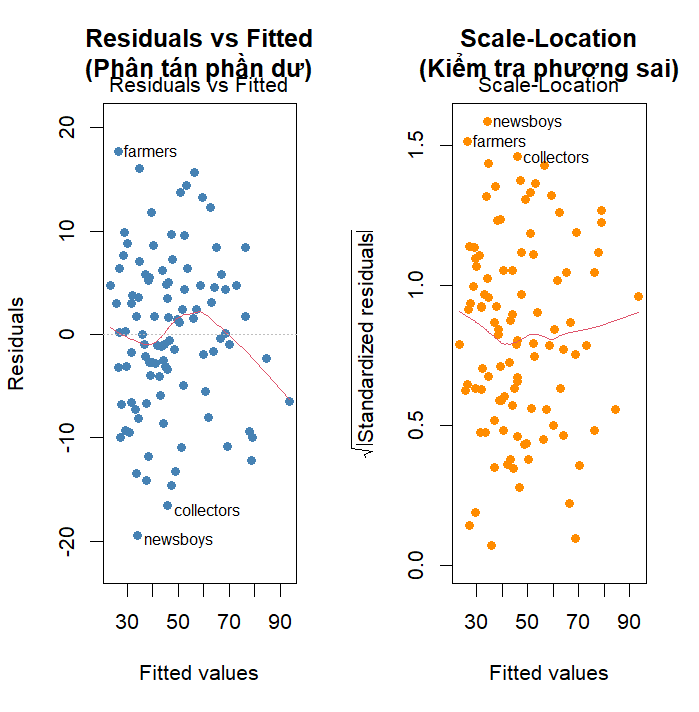
\includegraphics[width=0.8\textwidth]{1.png}
    \caption{Biểu đồ chẩn đoán cơ bản}
    \label{fig:Biểu đồ chẩn đoán cơ bản}
\end{figure}
Dựa vào ảnh trên, ta có thể thấy rằng đồ thị chẩn đoán gồm hai cấu phần độc lập đóng vai trò kiểm tra các giả định nền tảng của mô hình OLS gốc trước khi tiến hành suy diễn thống kê.\\
Đối với đồ thị bên trái: "Residuals vs Fitted" (Phân tán phần dư). Đồ thị này chủ yếu được sử dụng để thẩm định giả định A1 về tính tuyến tính và sàng lọc các quan sát ngoại lai có tầm ảnh hưởng lớn. Đặc tính hình học của đồ thị được thể hiện qua đường xu hướng màu đỏ (đường làm mịn dạng LOESS) vẽ xuyên qua đám mây phần dư. Về tổng thể, đường màu đỏ này bám tương đối sát và dao động xung quanh đường tham chiếu nét đứt $e = 0$ tại phân khúc tập trung mật độ dữ liệu cao (giá trị dự báo từ 30 đến 70). Tuy nhiên, khi giá trị dự báo vượt ngưỡng 70, đường xu hướng có xu hướng chúi xuống tương đối rõ nét. Sự lệch hướng ở phần đuôi này phát ra một chỉ dấu thực nghiệm về một sự vi phạm cục bộ đối với dạng hàm tuyến tính thuần túy ở các vùng biên dữ liệu cao. Thêm vào đó, thuật toán đồ thị đã tự động gắn nhãn định danh cho ba quan sát có phần dư cực đoan nhất trong mẫu: điểm farmers nằm cô lập ở phía trên đại diện cho sai số dương lớn (mô hình dự báo thấp hơn thực tế), trong khi hai điểm collectors và newsboys bị kéo mạnh xuống phía dưới đáy đồ thị biểu thị sai số âm nghiêm trọng (mô hình dự báo vượt quá xa thực tế).\\
Bên cạnh đó, đồ thị bên phải: "Scale-Location" (Kiểm tra phương sai) cung cấp bằng chứng trực quan định tính, đóng vai trò nền tảng củng cố cho kết quả của kiểm định White ($p = 0.02371$) về việc vi phạm giả định A3: Đồng nhất phương sai. Đồ thị biểu diễn mối quan hệ giữa căn bậc hai của giá trị tuyệt đối phần dư chuẩn hóa và giá trị dự báo. Nếu giả định đồng nhất phương sai được thỏa mãn, đường xu hướng màu đỏ bắt buộc phải là một đường thẳng nằm ngang hoàn hảo và đám mây dữ liệu phải phân tán đều đặn theo chiều thẳng đứng. Trái lại, đồ thị thực tế hiển thị đường màu đỏ uốn lượn hình sóng, ban đầu hơi võng xuống ở mức giá trị 40 và sau đó dốc ngược đi lên khi vượt quá mức 70.Đồng thời, cấu trúc hình học của các điểm dữ liệu cho thấy sự bất đối xứng nghiêm trọng về độ phân tán dọc. Tại phân khúc giá trị dự báo từ 30 đến 60, các điểm dữ liệu tạo thành một cột phương sai rất cao và dày đặc, bị đẩy lên đỉnh bởi các quan sát ngoại lai có độ biến động cực lớn đã được nhận diện là newsboys, farmers và collectors. Ngược lại, khi tiến về phía cuối trục hoành, mật độ điểm co cụm lại và biên độ phân tán dọc bị thay đổi hình thái. Hiện tượng đám mây phần dư phình-ngót không đều và đường xu hướng uốn cong này là một minh chứng hình học kinh điển cho thấy phương sai của sai số ngẫu nhiên bị phụ thuộc vào đại lượng dự báo. Nó bác bỏ hoàn toàn giả thuyết về một hằng số phương sai duy nhất, khẳng định mô hình đã mắc căn bệnh phương sai thay đổi do các tác động phi tuyến gây ra, và chứng minh việc bạn sử dụng liều thuốc sai số chuẩn vững HC3 ở đồ thị trước là một bước xử lý kỹ thuật hoàn toàn bắt buộc và chính xác.
\begin{figure}
    \centering
    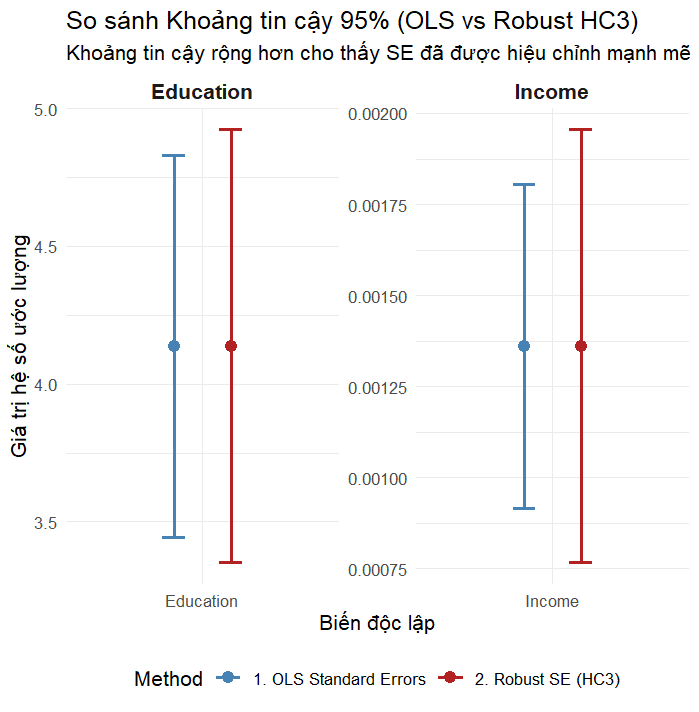
\includegraphics[width=0.8\textwidth]{2.png}
    \caption{Biểu đồ so sánh Khoảng tin cậy bằng ggplot2}
    \label{fig:Biểu đồ so sánh Khoảng tin cậy bằng ggplot2}
\end{figure}
Dựa vào ảnh trên, đồ thị so sánh khoảng tin cậy 95\% cung cấp một minh chứng trực quan rõ rệt cho giai đoạn khắc phục hiện tượng phương sai thay đổi trong quy trình phân tích. Đồ thị thực hiện so sánh các khoảng tin cậy của hệ số hồi quy được tính toán từ sai số chuẩn OLS truyền thống (màu xanh) và sai số chuẩn vững Huber-White hệ số hiệu chỉnh HC3 (màu đỏ) đối với hai biến độc lập là trình độ học vấn (Education) và thu nhập (Income).Đặc tính cốt lõi đầu tiên cần ghi nhận là vị trí của các điểm ước lượng (các chấm tròn biểu diễn hệ số $\hat{\beta}$) của cả hai phương pháp đều hoàn toàn trùng khớp nhau trên cùng một đường ngang. Đặc điểm này chứng minh một nguyên lý tảng băng trong kinh tế lượng: việc hiệu chỉnh sai số chuẩn vững không hề làm thay đổi giá trị của các hệ số hồi quy mẫu vốn đã đạt tính không chệch, mà nó chỉ tái định lượng độ biến động phân phối mẫu của chúng.Tuy nhiên, đặc tính kỹ thuật quan trọng nhất nằm ở chiều dài của các thanh sai số (error bars). Khoảng tin cậy màu đỏ của hệ số vững HC3 ở cả hai biến đều giãn rộng hơn một cách rõ rệt so với khoảng tin cậy màu xanh của OLS gốc. Khi mô hình tồn tại hiện tượng phương sai thay đổi, thuật toán OLS thông thường sẽ làm hạ thấp sai số chuẩn một cách sai lệch, từ đó bóp nghẹt khoảng tin cậy khiến người nghiên cứu rơi vào trạng thái "lạc quan giả tạo". Phép hiệu chỉnh HC3 đã trừng phạt và đẩy sai số chuẩn về đúng quy mô tiệm cận thực tế của nó, làm mở rộng khoảng tin cậy để phản ánh đúng mức độ rủi ro của dữ liệu. Điểm mấu chốt cuối cùng là dù khoảng tin cậy HC3 có bị kéo rộng ra, cả hai thanh sai số đều nằm hoàn toàn về một phía so với giá trị 0 (thanh của Education duy trì vị trí cao trên mức 3.0 và thanh của Income nằm hoàn toàn trên mức 0.00075). Điều này khẳng định kết luận trong bảng tổng hợp của bài báo cáo: sau khi chịu một cơ chế phạt nghiêm khắc từ HC3, tác động biên của thu nhập và học vấn đến uy tín nghề nghiệp vẫn giữ nguyên vẹn ý nghĩa thống kê tối cao ($***$).
	% ============================================================
	% DANH MỤC TÀI LIỆU THAM KHẢO (BIBLIOGRAPHY)
	% ============================================================
	\newpage
	\begin{thebibliography}{99}
		
		\bibitem{breusch1979} 
		Breusch, T. S., \& Pagan, A. R. (1979). 
		A simple test for heteroscedasticity and random coefficient variation. 
		\textit{Econometrica}, 47(5), 1287--1294.
		
		\bibitem{dobson2018} 
		Dobson, A. J., \& Barnett, A. G. (2018). 
		\textit{An Introduction to Generalized Linear Models} (4th ed.). 
		Chapman and Hall/CRC.
		
		\bibitem{faraway2016} 
		Faraway, J. J. (2016). 
		\textit{Linear Models with R} (2nd ed.). 
		Chapman and Hall/CRC.
		
		\bibitem{galton1886} 
		Galton, F. (1886). 
		Regression towards mediocrity in hereditary stature. 
		\textit{The Journal of the Anthropological Institute}, 15, 246--263.
		
		\bibitem{huber1967} 
		Huber, P. J. (1967). 
		The behavior of maximum likelihood estimates under nonstandard conditions. 
		\textit{Proceedings of the Fifth Berkeley Symposium}, 1, 221--233.
		
		\bibitem{james2013} 
		James, G., Witten, D., Hastie, T., \& Tibshirani, R. (2013). 
		\textit{An Introduction to Statistical Learning}. 
		Springer Science \& Business Media.
		
		\bibitem{koenker1981} 
		Koenker, R. (1981). 
		A note on studentizing a test for heteroscedasticity. 
		\textit{Journal of Econometrics}, 17(1), 107--112.
		
		\bibitem{mackinnon1985} 
		MacKinnon, J. G., \& White, H. (1985). 
		Some heteroskedasticity-consistent covariance matrix estimators with improved finite sample properties. 
		\textit{Journal of Econometrics}, 29(3), 305--325.
		
		\bibitem{maddala2001} 
		Maddala, G. S. (2001). 
		\textit{Introduction to Econometrics} (3rd ed.). 
		John Wiley \& Sons.
		
		\bibitem{rencher2008} 
		Rencher, A. C., \& Schaalje, G. B. (2008). 
		\textit{Linear Models in Statistics} (2nd ed.). 
		John Wiley \& Sons.
		
		\bibitem{sheather2009} 
		Sheather, S. (2009). 
		\textit{A Modern Approach to Regression with R}. 
		Springer Science \& Business Media.
		
		\bibitem{weisberg2014} 
		Weisberg, S. (2014). 
		\textit{Applied Linear Regression} (4th ed.). 
		John Wiley \& Sons.
		
		\bibitem{white1980} 
		White, H. (1980). 
		A heteroskedasticity-consistent covariance matrix estimator and a direct test for heteroskedasticity. 
		\textit{Econometrica}, 48(4), 817--838.
		
		\bibitem{wooldridge2015} 
		Wooldridge, J. M. (2015). 
		\textit{Introductory Econometrics: A Modern Approach} (6th ed.). 
		Cengage Learning.
		
	\end{thebibliography}
	
\end{document}